\documentclass[spanish,11pt,a4paper]{article}
\usepackage{recursos/paquetes}
\usepackage{recursos/modificaciones}

\begin{document}
	\maketitle
	{\small \textbf{Notita:} si hay algo mal o raro, decímelo así puedo corregirlo \emoji{winking-face}}
	\begin{multicols}{2}
\textcolor{white}{.}
	\vspace{-3cm}   
	\tableofcontents
	\end{multicols}
	\newpage
	\part{Introducción al diseño mecánico}
	\section{Diseño}
	\subsection{Conceptos básicos}
	\begin{itemize}
		\item Máquina: objeto utilizado para facilitar o realizar un trabajo determinado,	generalmente transformando una forma de energía en	movimiento o trabajo.
		\item Mecanismos: conjunto de piezas o elementos que ajustados entre sí y empleando energía mecánica
		hacen un trabajo o cumplen una función.
		\item Elemento de máquina: componente de una
		aplicación técnica que cumple una determinada función en las máquinas. Ejemplo
	\end{itemize}
	
	\subsection{Diseñar para construir}
	Es el término utilizado para vincular el diseño productivo —ingeniería de detalle—, de acuerdo con las instalaciones y procesos productivos con que cuenta un taller o fábrica
	de mecanizado. El proyectista no puede desarrollar una ingeniería acorde sin el conocimiento de cómo será el proceso
	productivo para la construcción de una máquina o parte de esta.
	\\	
	De lo que entendí: mejorar el proceso productivo implica reducciones en los costos finales, menor pérdida de material, menor pérdida de tiempo en tareas que no agregan valor agregado al producto.
	\\
	Cuatro pilares de la ingeniería:
	\begin{itemize}
		\item Ciencia: Base teórica, leyes físicas, matemáticas, química, etc.
		
		\item Experiencia: Conocimiento práctico acumulado, lecciones aprendidas.
		
		\item Creatividad: Capacidad de encontrar soluciones innovadoras.
		
		\item Tecnología: Herramientas, procesos y metodologías aplicadas para resolver problemas.
	\end{itemize}
	Otras posibles opciones para el cuarto pilar (porque no me acuerdo cuál era), dependiendo del enfoque:
	\begin{itemize}
	\item Ética: Consideraciones humanas, sociales y ambientales.
	\item Gestión: Organización, liderazgo y toma de decisiones.
	\end{itemize}
	
	\subsection{Diseño}
	
	Planificación para solver una necesidad.
	
	Etapas:
	\begin{itemize}
		\item Planificación y planteamiento
		\item Estrategia y análisis
		\item Diseño del concepto
		\item Diseño de detalle
		\item Prototipado e industrialización
	\end{itemize}
	
	\subsubsection{Consideraciones de diseño}
	\begin{itemize}
		\item Condiciones de trabajo
		\item Propiedades del material
		\item Características geométricas
		\item Comercialización
		\item Mantenimiento
		\item Responsabilidad legal
	\end{itemize}
	
	\section{Seguridad}
	\subsection{Coeficiente de seguridad}
	Método para tener un margen entre la carga aplicada y la resistencia del material:
	
	\[CS = \dfrac{resistencia}{esfuerzo}\]
	
	En función de los esfuerzos se expresa como:
	\[CS =  \dfrac{S}{\sigma_\text{adm}}\]
	
	Para materiales dúctiles la tensión de fallo corresponde la tensión de fluencia $S_f$. Mientras que, para materiales frágiles, es la tensión de rotura $S_r$.
	
	\subsubsection{Incertidumbre}
	
	La incertidumbre hace referencia a aquellos factores no contemplados de manera explícita en el proceso de cálculo del diseño mecánico, los cuales pueden afectar el resultado final o el comportamiento del sistema. Los tipos de incertidumbres se agrupan en cinco categorías:
	\begin{itemize}
		\item Incertidumbre de la carga actuante
		\item Resistencia del material
		\item Relación de las cargas aplicadas y la resistencia del material
		\item Consecuencia de la falla, cómo afecta la seguridad humana y la economía
		\item Costo relacionado con el aumento del $CS$
	\end{itemize}
	
	\subsection{Ensayo de tracción}
	Consiste en someter una probeta a un esfuerzo de tracción simple y representar gráficamente el valor del \emph{esfuerzo} aplicado en función de la \emph{deformación unitaria}. A partir de este ensayo se obtienen cinco datos relevantes:
	\begin{itemize}
		\item Tensión última o de rotura: es el valor máximo de tensión alcanzado antes de que la probeta se fracture.
		\item Límite elástico ($S_f$): es el esfuerzo normal hasta el cual la curva tensión-deformación se comporta de manera lineal. También se lo conoce como tensión de fluencia. Si el ensayo se interrumpe antes de alcanzar este punto, la probeta puede recuperar su forma original —comportamiento elástico—. En caso contrario, la probeta quedará deformada permanentemente —comportamiento plástico—.
		\item Módulo de elasticidad ($E$): es la pendiente de la zona lineal de la curva, y representa la relación entre la tensión aplicada y la deformación unitaria.
		\item Resiliencia: cantidad de energía absorbida por el material en la zona elástica.
		\item Tenacidad: energía total absorbida por el material hasta el punto de rotura.
	\end{itemize}
	
	La curva tensión-deformación puede dividirse en dos zonas bien diferenciadas, y el área bajo la curva representa la energía absorbida por el material:
	\begin{itemize}
		\item Zona elástica
		\item Zona plástica
	\end{itemize}
	
	\subsubsection{Diferencias entre materiales frágiles y dúctiles}
	
	Los materiales frágiles se caracterizan por no presentar zona plástica apreciable: se fracturan casi inmediatamente después de alcanzar su límite elástico. Tienen alta resistencia a la rotura pero baja capacidad de deformación. La energía absorbida antes de la fractura es baja, lo que se traduce en una baja tenacidad. Además, suelen romperse de forma repentina y sin señales visibles de deformación previa.
	
	En cambio, los materiales dúctiles exhiben una amplia zona plástica. Pueden deformarse considerablemente antes de romperse, lo que les otorga una alta tenacidad. Presentan una menor resistencia a la rotura comparados con los frágiles, pero tienen mayor capacidad de absorber energía y de advertir fallas mediante deformaciones visibles.

	
	\subsection{Proyecto mecánico}
	
	\begin{itemize}
		\item Planteamiento del problema
		\item Diseño o dimensionamiento de las partes
		\item Documentación técnica
		\item Ensayos y pruebas
		\item Reingeniería
	\end{itemize}
	
	Debe mantener un equilibrio entre los siguientes aspectos:
	\begin{itemize}
		\item Técnico
		\item Económico
		\item Ambiental
		\item Social
	\end{itemize}
	
	\part{Cargas, árboles y ejes}
	
	\section{Prevención de fallas}
	
	\subsection{Círculo de Mohr}
	
	Se utiliza para representar el estado de esfuerzos en un punto. Permite calcular:
	\begin{itemize}
		\item Los esfuerzos en un estado (normales $\sigma_{x}$, $\sigma_y$ y cortantes $\tau_{xy}$).
		\item Los esfuerzos principales ($\sigma_{1,2,3}$).
		\item El esfuerzo cortante máximo ($\tau_\text{máx}$).
		\item La orientación de los planos principales y de los planos de esfuerzo cortante máximo ($\theta$).
	\end{itemize}
	
	El eje de abscisas representa el esfuerzo normal ($\sigma$), positivo a tracción. Las ordenadas representan el esfuerzo cortante ($\tau$), positivo en sentido horario.\\
	
	La circunferencia se grafica teniendo en cuenta su centro y radio, y se calculan como sigue:
	\begin{align*}
		C &= \dfrac{\sigma_x + \sigma_y}{2}\\
		R &= \sqrt{\left(\dfrac{\sigma_x - \sigma_y}{2}\right)^2 + \tau_{xy}^2}
	\end{align*}
	\begin{figure}[h]
		\centering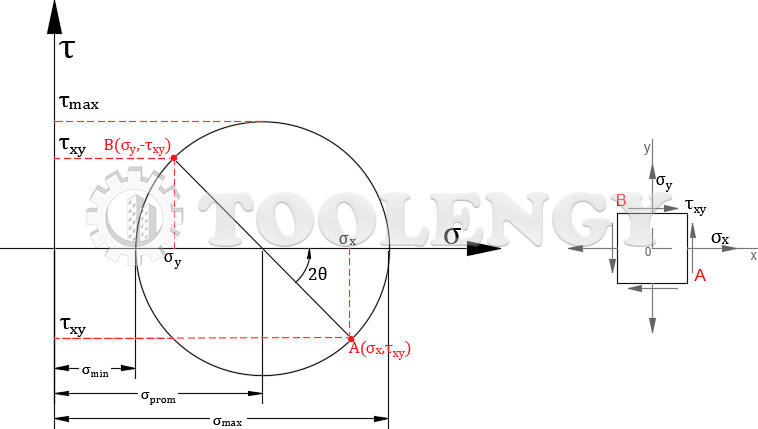
\includegraphics[width=.9\linewidth]{mohr}
	\end{figure}
	
	\subsubsection{Esfuerzos principales}
	
	Los esfuerzos principales se presentan cuando el esfuerzo cortante es nulo. En el círculo de Mohr, se ubican en los extremos horizontales. Se calculan mediante:
	
	\begin{align*}
		\sigma_{1,2} &= C \pm R \\
		\sigma_{1,2} &= \dfrac{\sigma_x + \sigma_y}{2} \pm \sqrt{\left(\dfrac{\sigma_x - \sigma_y}{2}\right)^2 + \tau_{xy}^2}
	\end{align*}
	
	\subsubsection{Esfuerzos cortantes máximos}
	
	Los esfuerzos cortantes máximos ocurren en planos orientados a 45° respecto de los planos principales. En el círculo de Mohr, se encuentran en los extremos verticales, y el esfuerzo normal correspondiente es igual al valor medio:
	\[\tau_{\text{máx},\text{mín}} = \pm  \sqrt{\left(\dfrac{\sigma_x - \sigma_y}{2}\right)^2 + \tau_{xy}^2}\]
	
	\subsubsection{Ensayo de tracción simple}
	
	En este ensayo, la probeta se somete a un esfuerzo uniaxial, por lo que sólo existe un esfuerzo principal: el máximo $\sigma_1$, que será igual a la tensión de fluencia del material —se toma este límite porque a partir de este punto la pieza pierde utilidad—. El esfuerzo normal máximo es la tensión de fluencia, y el esfuerzo cortante máximo es la mitad del anterior:
	\begin{align*}
		\sigma_\text{máx} &= S_f \\
		\tau_\text{máx} &= \tau_f = \dfrac{S_f}{2}
	\end{align*}
	  
	  \begin{figure}[h]
	  	\centering\caption{Círculo de Mohr en el ensayo de tracción simple.}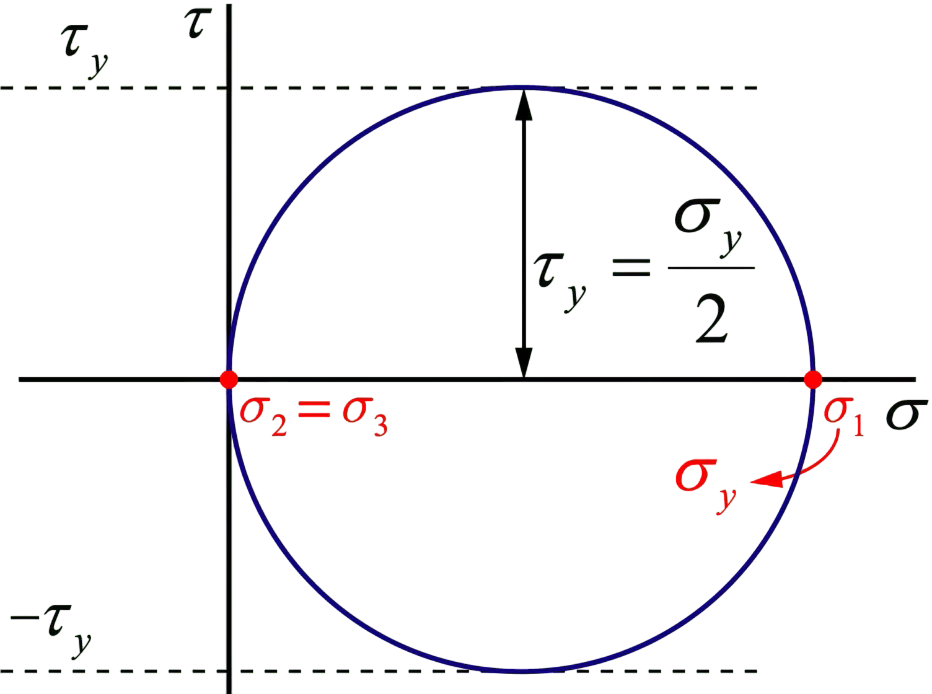
\includegraphics[width=.4\linewidth]{mohr-ensayo-traccion}
	  \end{figure}
	  
	  \begin{figure}[h]
	  	\centering\caption{Puntos importantes sobre la curva tensión-deformación para un material dúctil.}
	  	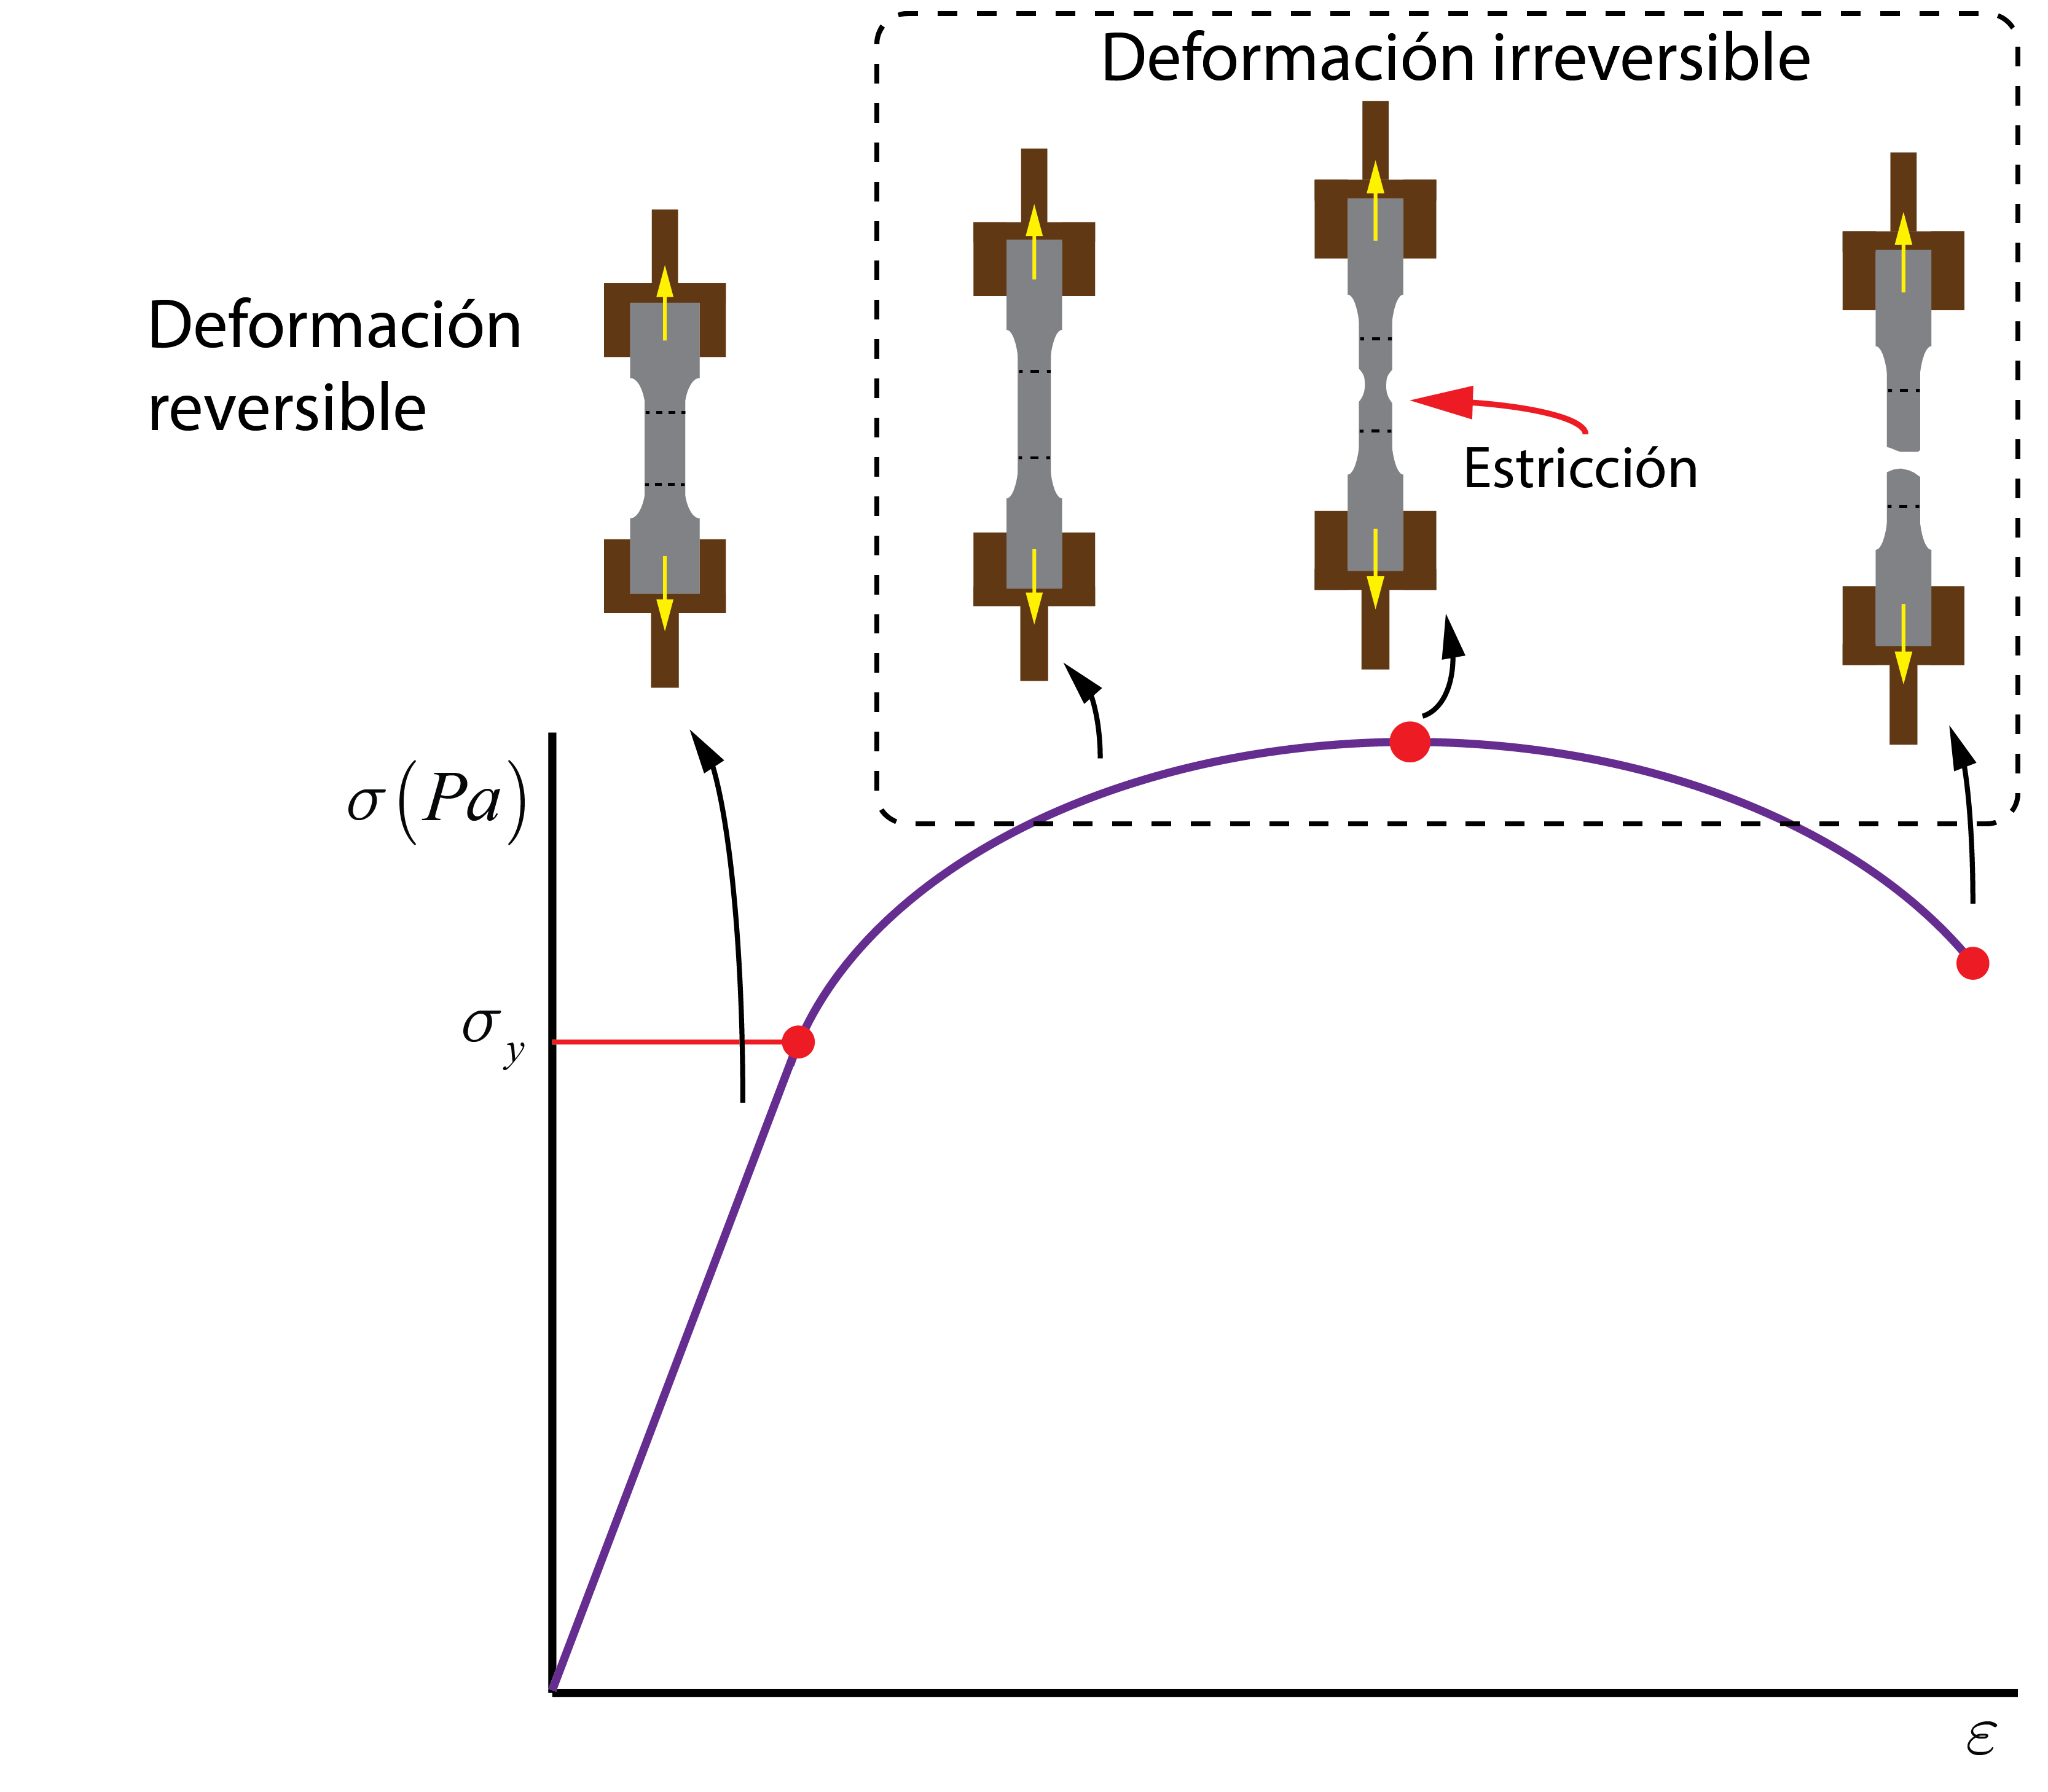
\includegraphics[width=.7\linewidth]{traccion-1}
	  \end{figure}
	  \begin{figure}[h]
	  	\centering
	  		\caption{Diferencias entre las curvas de materiales frágiles y dúctiles}
	  	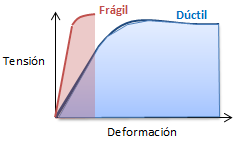
\includegraphics[width=.5\linewidth]{traccion-2}
	  	
	  \end{figure}
	
	\subsection{Tipos de fallas}
	
	La fractura puede clasificarse como \emph{dúctil} o \emph{frágil}, dependiendo del tipo de material, aunque también influyen otras condiciones. En general, la fractura dúctil se caracteriza por una deformación plástica significativa antes de la rotura. Presenta una superficie cónica en la rotura, resultado de la estricción. La fractura frágil es casi instantánea y sin deformación aparente. Es típica de materiales frágiles y se produce sin previo aviso.\\
	
	Sin embargo, en determinadas condiciones —por ejemplo, en fatiga— los materiales dúctiles pueden sufrir fracturas de tipo frágil, especialmente si hay defectos o grietas que reducen su tenacidad.
	
	
	\begin{figure}[h]
		\centering
		\caption{Fractura tipo dúctil —izquierda— y frágil —derecha—.}
		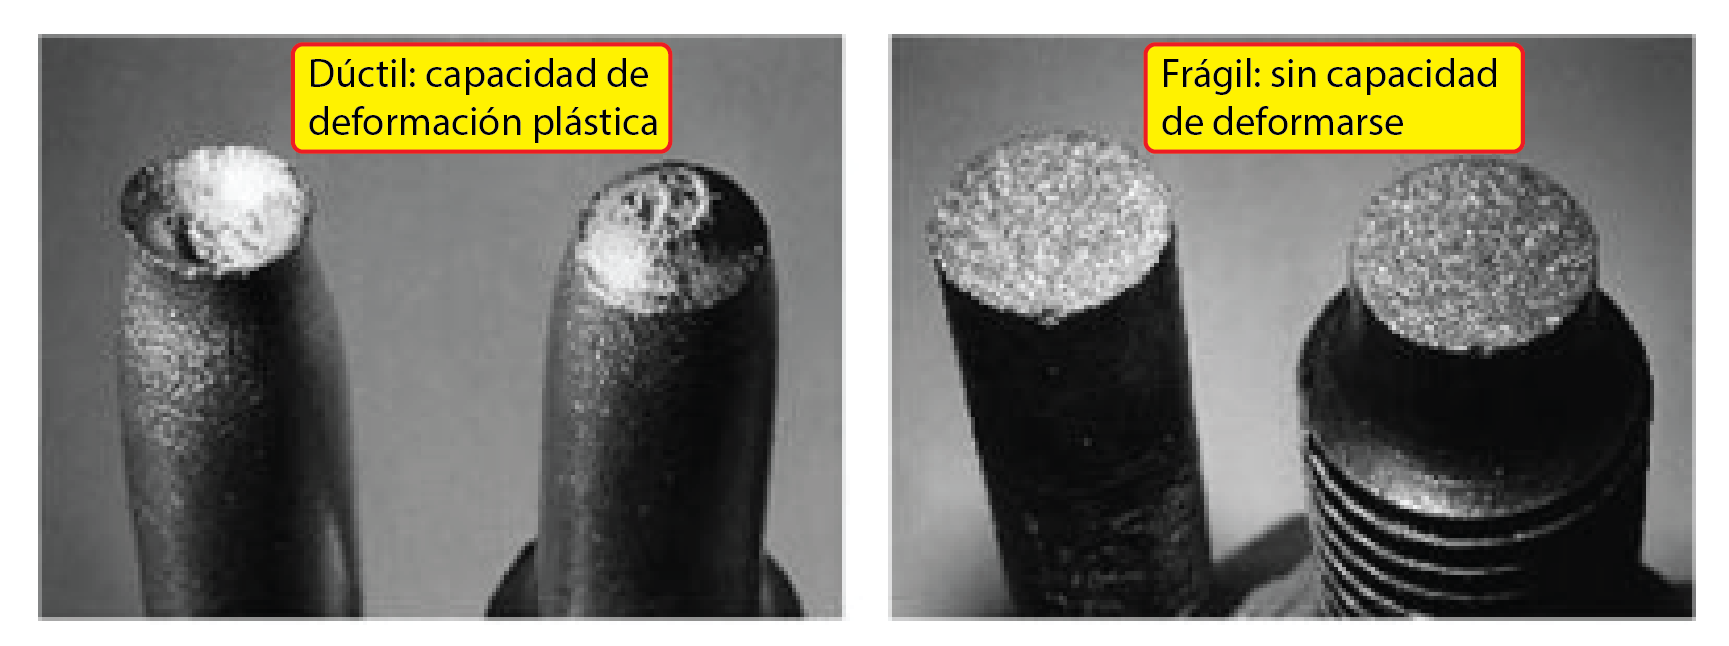
\includegraphics[width=.7\linewidth]{fractura}
	\end{figure}
	
	\subsection{Teorías de fallas}
	Las teorías de fallas se utilizan para predecir el tipo de falla que puede ocurrir en un material sometido a \emph{carga estática}, en función de su naturaleza y del tipo de esfuerzo aplicado. No existe una única teoría universal. Shigley presenta seis teorías, pero a continuación se muestran únicamente las vistas en clases.
	
	
	Todas las teorías comparan
	\begin{figure}[h]
		\centering
		\begin{tikzpicture}[node distance=2cm]
			% Nodos
			\node[draw, rectangle] (estado1) {un estado tensional};
			\node[draw, rectangle, right=of estado1] (estado2) {el estado en el ensayo de tracción simple};
			
			% Flecha
			\draw[-{Latex}] (estado1) -- node[above] {con} (estado2);
		\end{tikzpicture}
	\end{figure}
%	\begin{figure}[h]
%		\centering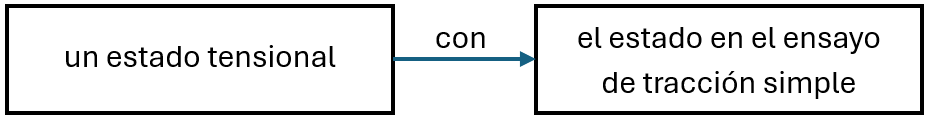
\includegraphics[width=.5\linewidth]{comparacion}
%	\end{figure}
	
	Es decir, relacionan los esfuerzos principales\footnote{En este documento solo se consideran estados de esfuerzo \emph{biaxiales}, ya que no se vieron con detalle los sistemas triaxiales.} $\sigma_1$ y $\sigma_2$ con los resultados obtenidos en dicho ensayo.%
	
	
	
	Para materiales frágiles se utilizan:
	\begin{itemize}
		\item Teoría de la máxima tensión normal.
		\item Teoría de la máxima deformación.
	\end{itemize}
	
	Para materiales dúctiles se utilizan:
	\begin{itemize}
		\item Teoría de la máxima tensión cortante.
		\item Teoría de la energía de distorsión.
	\end{itemize}
	
	En todas las teorías se debe aplicar un coeficiente de seguridad sobre las tensiones admisibles. Es decir, la tensión equivalente calculada según la teoría correspondiente ($\sigma$) debe ser menor o igual al límite del material ($S$) dividido por el coeficiente de seguridad:
		 \[\sigma \leq \dfrac{S}{CS}\]
		 
	Pero, a modo de simplificación, yo lo voy a dejar expresado sin el coeficiente de seguridad \emoji{slightly-smiling-face}
	
	% Materiales frágiles
	\subsubsection{Teoría de falla del esfuerzo normal máximo (ENM)}
	Presentada por Rankine. Indica que el fallo tendrá lugar cuando uno de los esfuerzos principales alcance el valor de la tensión de rotura.
	\begin{tcolorbox}
		\begin{equation*}
			\begin{aligned}
			\sigma_1 &\leq S_r \\
			\sigma_2 &\leq -S_r
			\end{aligned}
		\end{equation*}
	\end{tcolorbox}
	
	Se deberán comparar los valores obtenidos, y según el signo de cada uno, se deberán comparar con la resistencia a tracción o compresión del material.
	
	
	Si ambos resultados tienen el mismo signo, se tomará el de mayor valor absoluto. Si son positivos, se lo comparará con la resistencia a tracción, y si son negativos, con la resistencia a compresión. En cambio, si los valores tienen signos opuestos, cada uno se comparará con la tensión admisible correspondiente.
	
	Según un estado biaxial de esfuerzos, la teoría se expresa como:
	\begin{impo}[Teoría de falla del esfuerzo normal máximo]
		\begin{equation*}
			\dfrac{\sigma_x + \sigma_y}{2} \pm \sqrt{\left(\dfrac{\sigma_x - \sigma_y}{2}\right)^2 + \tau_{xy}^2} \leq \pm S_r
		\end{equation*}
	\end{impo}
	En la ecuación anterior, $+S_r$	representa la resistencia a la tracción, mientras que $−S_r$ corresponde a la resistencia a la compresión. \\
	
	
	Esta teoría no se utiliza para materiales dúctiles debido a su imprecisión, ya que el fallo sucede a tensiones mucho menores que la de fluencia.
	
	\subsubsection{Teoría de falla de la máxima deformación}
	
	La rotura ocurre cuando el alargamiento específico máximo en un punto alcanza el valor crítico de alargamiento específico que provoca la rotura en el ensayo de tracción simple, el cual se expresa como $\varepsilon = \sigma/E$.
	
	La condición de rotura se evalúa a partir de las deformaciones específicas máximas que se desarrollan en las direcciones principales. Para un estado plano de tensiones, se calculan mediante:
	\begin{equation*}
		\varepsilon_{1,2} = \dfrac{\sigma_{1,2}}{E} - \mu \dfrac{\sigma_{2,1}}{E}
	\end{equation*}
	donde $\mu$ es el coeficiente de Poisson.
	
	A continuación, se comparan dichas deformaciones principales con la deformación obtenida en el ensayo de tracción $\varepsilon_\text{ensayo}=\varepsilon_{1,2}$ y se llega a:
	\begin{impo}[Teoría de la máxima deformación]
		\begin{equation*}
		\dfrac{1-u}{2} (\sigma_x + \sigma_y) \pm \dfrac{1+u}{2} \sqrt{(\sigma_x - \sigma_y)^2 + 4 \tau_{xy}^2} \leq \pm S_r
		\end{equation*}
	\end{impo}
	% Materiales dúctiles
	\subsubsection{Teoría de falla del esfuerzo cortante máximo (ECM)}
	Esta teoría, propuesta por Tresca, establece que la fluencia comienza cuando la tensión cortante máxima alcanza el valor de la tensión cortante máxima observada en el ensayo de tracción simple:
	\[\tau_\text{máx} = \tau_f\]
	
	Según el círculo de Mohr, la tensión cortante máxima corresponde al radio del círculo:
	 $\dfrac{\sigma_1-\sigma_2}{2} = \tau_\text{máx}$. 
	 
	 En el ensayo de tracción simple, se tiene que $\sigma_2 = 0$ y $\sigma_1 = S_f$, por lo tanto:
	\begin{tcolorbox}
		\begin{equation*}
			\sigma_1 - \sigma_2 \leq S_f
		\end{equation*}
	\end{tcolorbox}
	Esta relación también puede expresarse en función de un estado biaxial:
	\begin{equation*}
		\begin{aligned}
			\tau_\text{máx} &=  \sigma_1 - \sigma_2 \\
			&= (C+R)-(C-R) = 2\,R \\
			&= \sqrt{(\sigma_x - \sigma_y)^2 + 4\, \tau_{xy}^2}
		\end{aligned}
	\end{equation*}
	Finalmente, la condición de fluencia según el criterio de Tresca se expresa como:
	\begin{impo}[Teoría de falla del esfuerzo cortante máximo]
		\begin{equation*}
			\sqrt{(\sigma_x - \sigma_y)^2 + 4\, \tau_{xy}^2} \leq S_f
		\end{equation*}
	\end{impo}
	
	\subsubsection{Teoría de falla de la energía de distorsión (ED)}
	La famosa teoría de Von Mises establece que la fluencia ocurre cuando la energía de distorsión alcanza el valor de la energía de distorsión obtenida en el ensayo de tracción simple.
	
	La energía de distorsión se calcula mediante la siguiente expresión:
	\[u_d = \dfrac{1+\mu}{6\,E} \left[(\sigma_1 - \sigma_2)^2 + (\sigma_2 - \sigma_3)^2 + (\sigma_3 - \sigma_1)^2\right]\]
	En el caso del ensayo de tracción uniaxial, donde $\sigma_1 = S_f$ y $\sigma_2=\sigma_3=0$, la energía de distorsión es: \[u_{d,\text{ensayo}} = \dfrac{1+\mu}{3\, E}S_f^2\]
	Igualando ambas expresiones se obtiene la condición de fluencia según Von Mises:
	\begin{tcolorbox}\begin{equation*}
			\sqrt{\dfrac{(\sigma_1 - \sigma_2)^2 + (\sigma_2 - \sigma_3)^2 + (\sigma_3 - \sigma_1)^2}{2}} \leq  S_f
		\end{equation*}
	\end{tcolorbox}
	El término del lado izquierdo se denomina \emph{tensión equivalente de Von Mises}, y se simboliza como $\sigma'$.
	
	En el caso de un estado biaxial de tensiones, la expresión es:
	\begin{impo}[Teoría de falla de la energía de distorsión]
		\begin{equation*}\sqrt{\sigma_x^2 - \sigma_x \sigma_y + \sigma_y^2 + 3\, \tau_{xy}^2}\leq S_f
		\end{equation*}
	\end{impo}
	\subsection{Fatiga}
	La fatiga es un tipo de falla que ocurre debido a la propagación progresiva de una grieta en el material, causada por cargas cíclicas o repetidas. Supone una reducción de la resistencia mecánica de los materiales cuando actúan cargas cíclicas o fluctuantes. Esta rotura se produce a niveles de tensión inferiores al límite elástico determinado en un ensayo de tracción simple.
	
	
	En la industria, se estima que alrededor del 80\% de las fallas en componentes mecánicos se deben a mecanismos de fatiga.
	
	Se utilizan tres enfoques principales del diseño y el análisis, para predecir cuándo, si alguna
	vez sucede, un componente de máquina cargado en forma cíclica fallará por fatiga durante
	un determinado periodo. Los tres métodos más importantes de fatiga-vida que se usan en el diseño y el análisis son el \emph{método de esfuerzo-vida}, el \emph{método de deformación-vida} y el \emph{método de mecánica de la fractura lineal elástica}.
	\begin{itemize}
		\item \emph{Método de esfuerzo-vida}: se basa sólo en niveles de esfuerzo, es el enfoque menos
		exacto, especialmente para aplicaciones de bajo ciclaje. Sin embargo, es el más fácil de implementar para una amplia variedad de aplicaciones de diseño, tiene una gran cantidad de datos de soporte y representa de manera adecuada las aplicaciones de alto ciclaje. En este se obtiene el diagrama $S$-$N$, y el dispositivo de ensayo a la fatiga que se emplea con más frecuencia es la máquina de viga rotativa de alta velocidad de R.R. Moore. Shigley organiza a este método en tres categorías: \begin{itemize}
			\item Carga completamente reversible: se ve el diagrama $S$-$N$, los factores que modifican el límite ed resistencia y la concentración de esfuerzos.
			\item Carga fluctuante: se ven los criterios de falla por fatiga.
			\item Combinaciones de modo de carga: acá se aplica la teoría ED + algún criterio de falla por fatiga.
		\end{itemize}
		
		\item \emph{Método de deformación-vida}: implica un análisis de la deformación
		plástica en regiones localizadas donde se considera a los esfuerzos y deformaciones para
		la estimación de la vida.Bueno para aplicaciones con fatiga	de bajo ciclaje.
		
		\item \emph{Método de la mecánica de la fractura}: supone que ya existe una grieta y que ésta
		se ha detectado. Se emplea para predecir el crecimiento de la grieta con respecto a
		la intensidad del esfuerzo.
	\end{itemize}
	\subsection{Cargas variables}
	
	Cargas variantes en el tiempo. Exiten los siguientes tipos (\autoref{fig:variable}):
	\begin{itemize}
		\item Alternativo o completamente invertido: donde $\sigma_m = 0$ y $\sigma_\text{máx} = - \sigma_\text{mín}$
		\item Intermitente o repetido: donde un extremo ($\sigma_\text{máx}$ o $\sigma_\text{mín}$) es nulo y $\sigma_m \neq 0$
		\item Variable o fluctuante: es el caso más general\footnote{En realidad, el caso más general sería donde hay dos amplitudes, pero no lo menciono acá.}.
	\end{itemize}
	\begin{figure}[h]
		\centering\caption{Algunas relaciones esfuerzo-tiempo.}\label{fig:variable}
		\begin{subfigure}{.44\linewidth}
		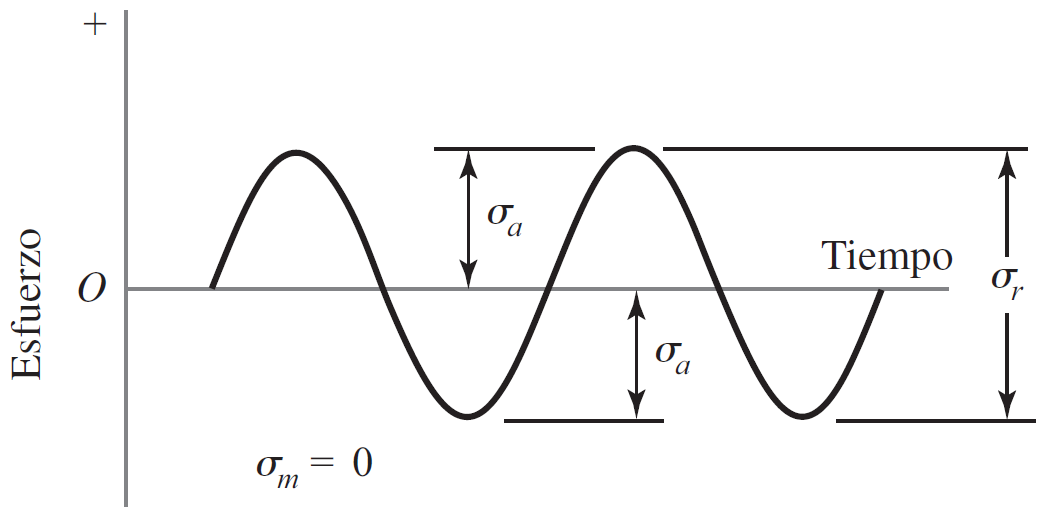
\includegraphics[height=3cm]{alternante}\caption{Esfuerzo alternante}
		\end{subfigure}
		\begin{subfigure}{.44\linewidth}
		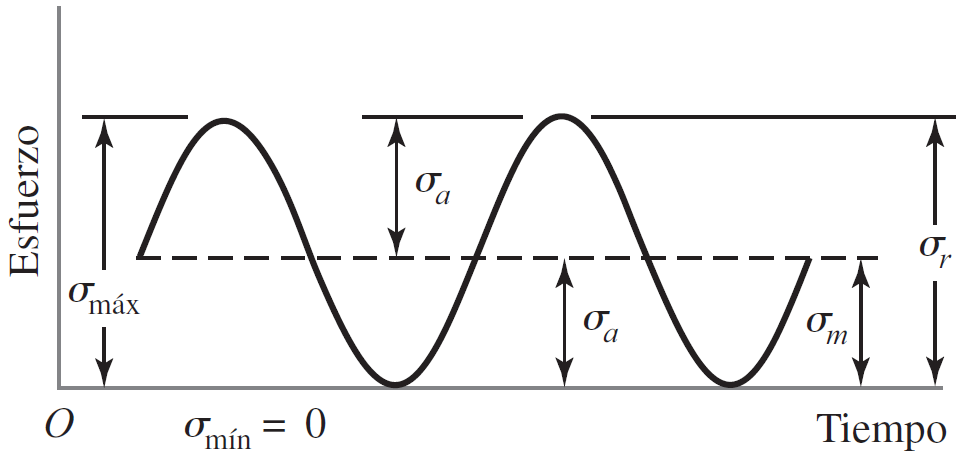
\includegraphics[height=3cm]{repetido}\caption{Esfuerzo repetido}
		\end{subfigure}
		
		\begin{subfigure}{.3\linewidth}
		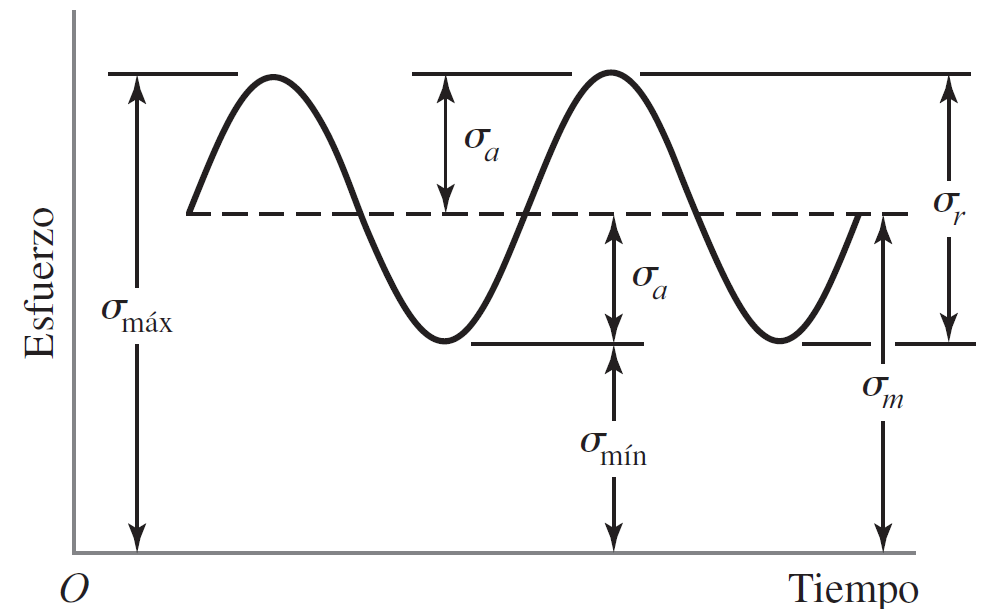
\includegraphics[width=\linewidth]{fluctuante}\caption{Esfuerzo variable}
		\end{subfigure}
	\end{figure}
	Parámetros de las tensiones en régimen variable:
	\begin{itemize}
		\item $\sigma_\text{mín}$ tensión mínima
		\item $\sigma_\text{máx}$ tensión máxima
		\item $\sigma_a$ amplitud de la tensión
		\item $\sigma_m$ tensión media o promedio
		\item $\sigma_r$ rango de la tensión
	\end{itemize}
	
	\subsection{Tensión límite de fatiga}
	
	Cuando un material dúctil está sometido a cargas cíclicas, puede fallar a tensiones menores que su límite de fluencia. A esta tensión se la denomina tensión límite de fatiga.
	
	
	Se define como el esfuerzo máximo que un material puede soportar durante un número infinito de ciclos sin fallar. Este valor depende tanto del nivel de esfuerzo como de la cantidad de ciclos, y se analiza mediante el \emph{diagrama $S$-$N$} (esfuerzo–número de ciclos).
	
	\subsubsection{Ensayo de flexión rotatoria}
	
	Los resultados del ensayo se representan en las llamadas curvas $S$-$N$, donde el eje vertical muestra la amplitud de tensión aplicada ($S$) y el eje horizontal, el logaritmo del número de ciclos hasta la rotura ($N$).
	
	
	En estos ensayos se registra cuántos ciclos resiste la probeta para cada nivel de tensión completamente invertidas\footnote{El esfuerzo se alterna entre magnitudes iguales de tensión y compresión.}. Las curvas muestran que la resistencia a fatiga aumenta cuando disminuye el número de ciclos, y disminuye cuando aumentan los ciclos aplicados.
	
	
	El límite inferior horizontal del diagrama representa el \emph{límite de fatiga} ($S_e'$). Si la tensión aplicada es menor a este valor, el material tendría \emph{vida infinita} y no fallaría por fatiga.
	\begin{figure}[h]
		\centering\caption{Diagrama $S$-$N$ que se graficó a partir de los resultados de ensayos a la fatiga axial completamente invertidos.}\label{fig:s-n}
		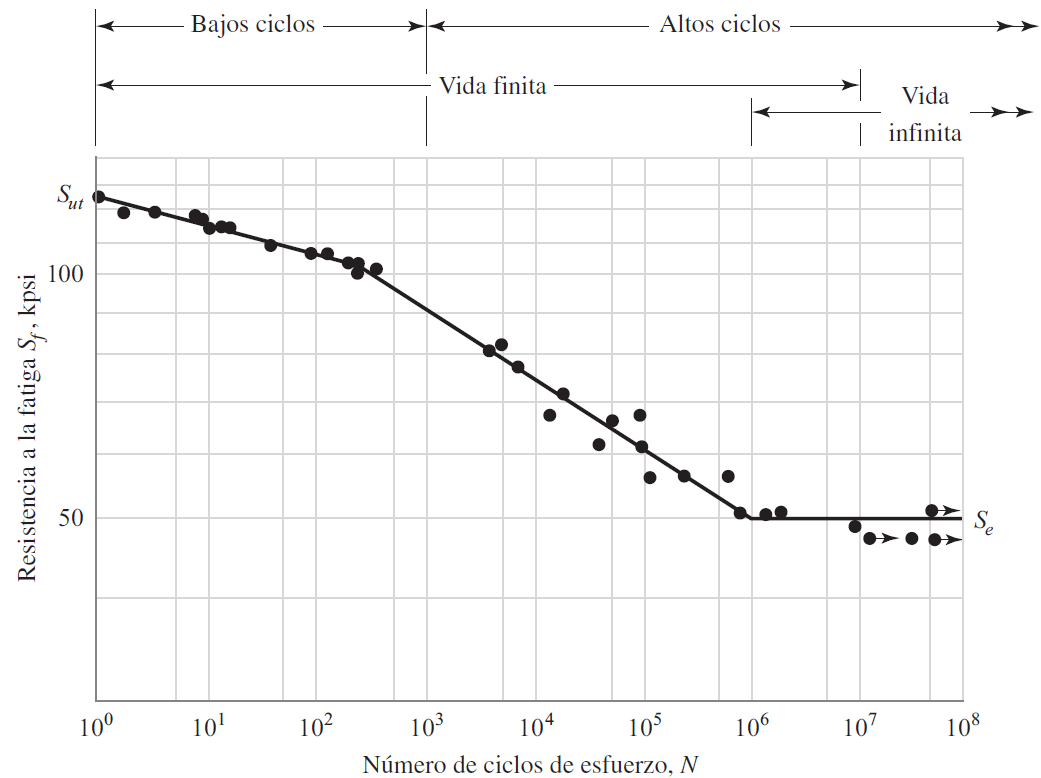
\includegraphics[width=.8\linewidth]{s-n}
	\end{figure}
	\begin{itemize}
		\item Para $N = 10^3$ ciclos, la rotura ocurre cuando $S = 0.9\,S_r$, siendo $S_r$ el límite de rotura.
		\item Para $N = 10^6$ ciclos (vida infinita), se toma $S_e' = 0.5\,S_r$.
	\end{itemize}
	
	Se emplea $S_r$ en lugar del límite de fluencia, ya que en carga variable el material no experimenta deformación plástica previa.
	
	\subsection{Tensión límite de fatiga corregida}
	
	El límite de fatiga real de una pieza puede diferir significativamente del obtenido en el diagrama $S$-$N$, ya que este se basa en ensayos ideales sobre probetas con geometría, acabado superficial y condiciones específicas, distintas a las reales.
	
	Para tener en cuenta estos factores, se corrige el valor de $S_e'$ aplicando coeficientes modificativos, lo que permite estimar un \emph{límite de fatiga corregido} ($S_e$) acorde a las condiciones reales de trabajo:
	\begin{tcolorbox}
		\begin{equation*}
			S_e = S_e' \cdot k_a \cdot k_b \cdot k_c \cdot k_d \cdot k_e \cdot k_f \cdot k_g
		\end{equation*}
	\end{tcolorbox}
	
	\subsubsection{Factores modificativos}
	
	\begin{itemize}
		\item $k_a$ Factor de carga:		
		 corrige según si la carga es axial, flexión o torsión. Cargas más severas —como torsión— reducen el límite de fatiga. 
		\item $k_b$ Factor de superficie:		
		 superficies rugosas o con defectos tienden a iniciar grietas antes, por lo que este factor reduce el límite de fatiga.
		\item $k_c$ Factor de tamaño:		
		 componentes más grandes presentan más probabilidad de contener defectos internos o concentraciones de esfuerzo, reduciendo su resistencia.
		\item $k_d$ Factor de confiabilidad:		
		 ajusta el límite de fatiga según el nivel de confiabilidad deseado. A mayor confiabilidad, menor se asume el límite admisible.
		\item $k_e$ Factor por temperatura:		
		 considera el efecto de la temperatura de trabajo. Temperaturas elevadas pueden debilitar el material.
		\item $k_f$ Factor por vida esperada:		
		 se ajusta según el número de ciclos esperados si se desea un diseño con vida finita distinta a $10^6$ ciclos.
		\item $k_g$ Factor por efectos diversos:		
		 factor general para condiciones especiales no incluidas en los anteriores:\begin{itemize}
		 	\item Tensiones residuales
		 	\item Características direccionales del material
		 	\item Tratamientos térmicos
		 	\item Corrosión
		 	\item Recubrimientos y tratamientos superficiales
		 	\item Entorno
		 \end{itemize}
	\end{itemize}
	
	\subsection{Criterios de falla por fatiga}
	
	Los criterios de falla por fatiga se utilizan para predecir cuándo un componente de máquina sometido a cargas cíclicas fallará debido a la fatiga. A diferencia de la falla estática, la falla por fatiga no proporciona una advertencia visible, siendo repentina, total y peligrosa. Estos criterios forman parte de los métodos de fatiga-vida, específicamente el método de esfuerzo-vida.
	
	
	Los esfuerzos en fatiga se caracterizan por sus componentes alternantes ($\sigma_a$) y medias ($\sigma_m$). 
	
	\begin{figure}[h]
		\centering\caption{Diagrama de fatiga donde se proporcionan varios criterios de falla. Para cada criterio, los puntos ``sobre'' la curva respectiva	indican falla.}
		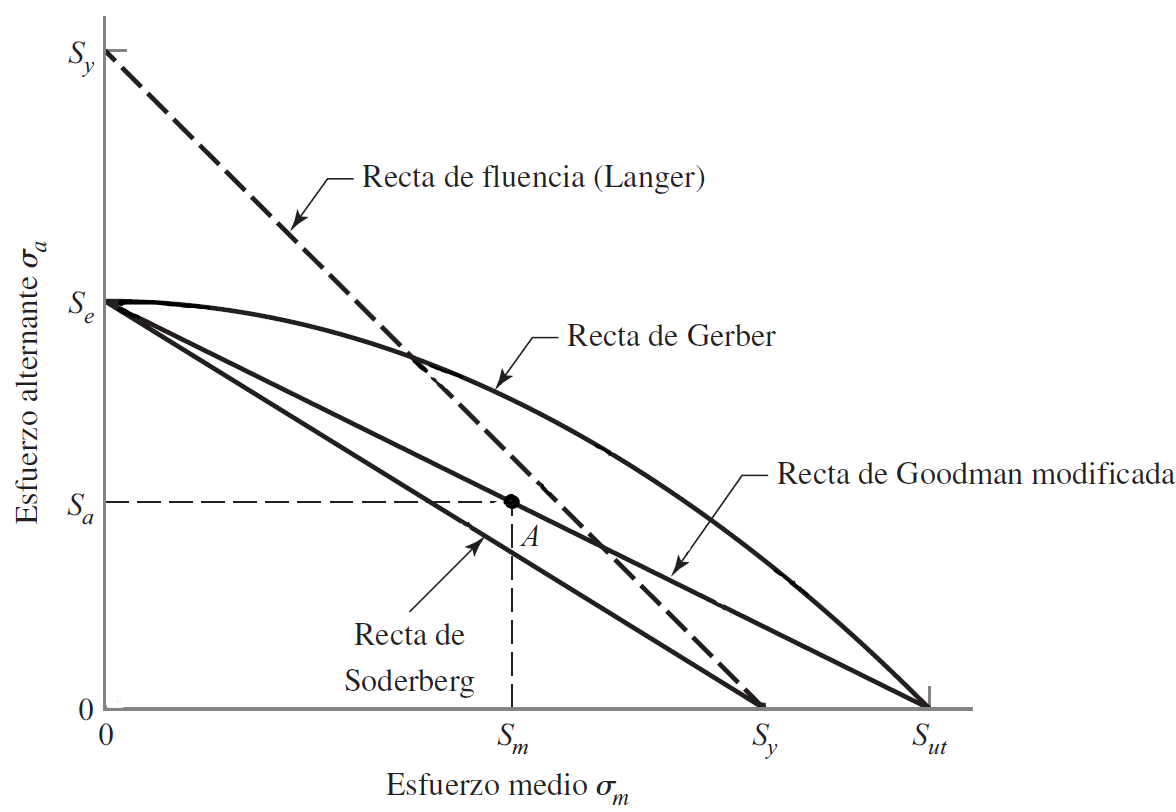
\includegraphics[width=.7\linewidth]{fatiga}
	\end{figure}
	
	\subsubsection{Criterio de Goodman}
	La ecuación de Goodman es: 
	\begin{tcolorbox}
		$$\dfrac{\sigma_a}{S_e} + \frac{\sigma_m}{S_{ut}} = \frac{1}{n}$$
	\end{tcolorbox}
	Se representa gráficamente como una línea recta. Aunque es fácil de usar y graficar, y permite discernir aspectos sutiles de la fatiga, se considera que no es conservador y no protege contra la fluencia en el primer ciclo (se ve que una zona se encuentra fuera de la zona de fluencia). Es ampliamente utilizado en el diseño y en análisis de falla.
	\subsubsection{Criterio de Soderberg}
	
	La ecuación de Soderberg solo reemplaza la resitencia última del criterio de Goodman con la resistencia a la fluencia: 
	\begin{tcolorbox}
		$$\dfrac{\sigma_a}{S_e} + \frac{\sigma_m}{S_f} = \frac{1}{n}$$
	\end{tcolorbox}
	Es el único criterio que ofrece protección contra la fluencia, ya que su curva de falla se mantiene conservadoramente dentro de la línea de fluencia (Langer\footnote{El objetivo principal de la línea de Langer es asegurar que el material no ceda plásticamente bajo la carga máxima aplicada durante el primer ciclo de operación.}). Se representa gráficamente como una línea recta.
	
	
	Tiende a ser más conservador que otros criterios.
	\subsubsection{Criterio de Gerber}
	La ecuación de Gerber es: 
	\begin{tcolorbox}
	$$\dfrac{n\,\sigma_a}{S_e} + \left(\dfrac{n\,\sigma_m}{S_{ut}}\right)^2 = 1$$
	\end{tcolorbox}
	
	Este criterio se ajusta mejor a los datos experimentales en comparación con Goodman, ya que pasa "por y entre los datos de fatiga". Se representa como una parábola.
	
	
	Al igual que Goodman, no protege contra la fluencia y requiere una verificación adicional para este modo de falla
	
	\section{Ejes y árboles}
	\subsection{Diferencias entre árboles y ejes}
	Una \emph{árbol} es un elemento rotatorio, generalmente de sección transversal circular, que se utiliza para \emph{transmitir potencia} o movimiento. Constituye el eje de rotación de componentes como engranes, poleas, volantes de inercia o manivelas, y además, controla la geometría de su movimiento.
	
	
	
	Un \emph{eje} es un elemento no giratorio que no transmite par de torsión y se emplea para \emph{soportar} ruedas rotatorias, poleas y elementos similares. Su diseño es más simple, asemejándose al análisis de una viga estática, y no requiere la atención especial que se da a los árboles giratorios sometidos a carga por fatiga.
	
	\subsection{Materiales y tratamientos térmicos}
	
	Materiales comúnmente utilizados y las consideraciones clave para su elección:
	
	Aceros de bajo carbono, estirados en frío y laminados en caliente:
	\begin{itemize}
	\item Muchos ejes se fabrican con aceros de bajo carbono, aceros estirados en frío o aceros laminados en caliente, como los aceros ANSI 1020 a 1050.
	\item La rigidez de un eje, representada por el módulo de elasticidad, es una propiedad esencialmente constante en todos los aceros, lo que significa que la rigidez no se puede controlar mediante la elección del material, sino solo a través de decisiones geométricas.
	\item La resistencia necesaria para soportar los esfuerzos de carga sí influye en la elección de los materiales y sus tratamientos.
	\end{itemize}
	
	Aceros para endurecimiento superficial:
	\begin{itemize}
	\item Los ejes no suelen requerir endurecimiento superficial a menos que sirvan como una superficie de contacto real.
	\item Las opciones típicas de material para el endurecimiento superficial incluyen los grados de carburización ANSI 1020, 4320, 4820 y 8620.
	\end{itemize}
	
	Tratamientos térmicos:
	\begin{itemize}
		\item Aumentan la dureza superficial mediante tratamientos térmicos como la cementación, nitruración o temple superficial, lo que mejora la resistencia al desgaste por fricción y prolonga la vida útil del eje.
		\item Incrementan la resistencia mecánica y la tenacidad mediante tratamientos como el normalizado o el temple y revenido, permitiendo que el eje soporte cargas elevadas de flexión y torsión sin fallar.
		\item Eliminan tensiones internas generadas durante el mecanizado mediante tratamientos térmicos de aliviado de tensiones, reduciendo el riesgo de deformaciones o fallas prematuras.
		\item Producen una superficie más lisa y homogénea a través de tratamientos como la normalización o el temple superficial —el pulido también es una solución—, disminuyendo la concentración de esfuerzos y mejorando el comportamiento frente a la fatiga.
	\end{itemize}
	
	
	
	Otros materiales y consideraciones:
	\begin{itemize}
		\item El acero inoxidable puede ser adecuado para ciertos entornos corrosivos.
		\item En general, la selección de un material para un componente de máquina, como un eje, es una de las decisiones más importantes para el diseñador. \textbf{No siempre se basa únicamente en el esfuerzo y la deflexión}. Otros factores como llenar espacios, estética, resistencia a la corrosión o efectos de temperatura pueden ser más relevantes.
	\end{itemize}
	
	
	
	\subsection{Dimensionamiento de ejes}
	\begin{enumerate}
		\item Se definen los componentes que montará el eje, así como su disposición general en el sistema.
		
		\item Se analizan los esfuerzos y la resistencia en las zonas críticas —donde se presentan grandes momentos flectores, pares de torsión o concentraciones de tensiones—. Los esfuerzos combinados se transforman en esfuerzos equivalentes de Von Mises, los cuales se comparan con criterios de fatiga, como el de Soderberg, tal como se hizo en el trabajo práctico.
		
		\item Una vez definidas las dimensiones tentativas, se evalúan la rigidez y la deflexión. Las deflexiones excesivas pueden generar velocidades críticas peligrosas, que inducen vibraciones y aceleran la falla de otros componentes.
		
		\item Finalmente, si se emplean criterios distintos al de Soderberg —como Gerber o Goodman—, se debe verificar adicionalmente la línea de Langer. Esta garantiza que el material no entre en régimen de fluencia plástica desde el primer ciclo de carga, aspecto que los criterios mencionados no contemplan de forma inherente.
	\end{enumerate}
	
	En cálculos, para el trabajo práctico, se siguió este procedimiento (Capítulo 6-18 del Shigley 9na edición), considerando \textbf{combinaciones de modos de carga}:
	
	\begin{enumerate}	
		\item Determinación de solicitaciones actuantes sobre el eje.
		\item Cálculo de límite de tensión de fatiga modificada ($S_e$):
		\begin{itemize}
			\item Límite de tensión de fatiga debido solamente a la rotación ($S_e'$).
			\item Factores modificativos.
		\end{itemize}
		\item Esfuerzos de Von Mises alternante ($\sigma_a$) y medio ($\sigma_m$)
		\item Aplicación del criterio de fatiga: una vez obtenidos los esfuerzos equivalentes, se aplica uno de los criterios de fatiga. Soderberg es el más conservador.
	\end{enumerate}
	
	
	\subsection{Componentes de un eje}
	Los componentes de un eje (árbol) y los elementos que se montan sobre el mismo, y los medios para asegurarlos o transmitir el par son:
	\begin{itemize}
	\item Engranajes: utilizados para transmitir movimiento y potencia, y a menudo son una fuente de las fuerzas que actúan sobre el eje.
	\item Poleas: empleadas para la transmisión de potencia, similar a los engranes.
	\item Volantes de inercia, manivelas, ruedas dentadas o catarinas y elementos similares: otros dispositivos que constituyen el eje de rotación u oscilación de la flecha.
	\item Cojinetes: soportan el eje y sus componentes, permitiendo la rotación. Pueden ser de contacto rodante o de contacto deslizante.
	\item Hombros o resaltos: cambios de diámetro en el eje que sirven para ubicar axialmente los componentes (como engranes y cojinetes) y para soportar cargas de empuje.
	\item Anillos de retención: se utilizan en ranuras cortadas en el eje para posicionar axialmente los componentes.
	\item Manguitos entre componentes: elementos utilizados para mantener la separación axial entre componentes montados en el eje.
	\item Collarines de sujeción: se emplean para mantener los componentes en una posición axial específica sobre el eje.
	\item Cuñas: elementos que se ajustan en ranuras del eje y del componente (engrane, polea) para transmitir el par de torsión y asegurar la orientación angular.
	\item Ejes estriados: una configuración del propio eje con dientes o formas que se acoplan con el diámetro interior de un componente para transmitir pares de torsión significativos y permitir el movimiento axial.
	\item Tornillos de fijación: se basan en la compresión para sujetar elementos al eje, proporcionando capacidad de sujeción axial y tangencial para resistir el par de torsión.
	\item Pasadores: usados para posicionar axialmente elementos y/o transferir par de torsión o empuje.
	\item Ajustes a presión o por contracción: métodos de montaje que utilizan la interferencia entre el eje y el componente para transmitir el par de torsión y asegurar la ubicación axial.
	\item Ajustes ahusados: permiten una sujeción firme del componente al eje, a menudo en los extremos sobresalientes.
	\item Tuercas: utilizadas para sujetar firmemente las ruedas al eje, especialmente con ajustes ahusados o para fijar cojinetes
	\end{itemize}
	
	\subsection{Factor de concentración de tensiones}
	
	\subsubsection{Factor de concentración de tensiones teórico}
		El factor teórico o geométrico de concentración de esfuerzos ($K_t$) se utiliza para \emph{relacionar el esfuerzo máximo real en una discontinuidad con el esfuerzo nominal}. Se define como la relación entre el esfuerzo máximo ($\sigma_{\text{máx}}$) y el esfuerzo nominal ($\sigma_0$) para esfuerzos normales, o entre el esfuerzo cortante máximo ($\tau_{\text{máx}}$) y el esfuerzo cortante nominal ($\tau_0$) para esfuerzos cortantes:
		\begin{equation*}
			K_t = \dfrac{\sigma_{\text{máx}}}{\sigma_0} \quad \text{y} \quad K_{ts} = \dfrac{\tau_{\text{máx}}}{\tau_0}
		\end{equation*}
		Su valor \emph{depende únicamente de la geometría de la pieza}, el material utilizado no tiene efecto en su valor.
		
		Los valores de $K_t$ o $K_{ts}$ se pueden encontrar en tablas y gráficas para diversas geometrías.
	\subsubsection{Factor de concentración de tensiones}
	Es un valor reducido de $K_t$ (o $K_{ts}$ para cortante) que se utiliza en el análisis de fatiga. Se introduce porque algunos materiales no son completamente sensibles a la presencia de muescas. Esto significa que el esfuerzo máximo real bajo cargas de fatiga puede ser menor que el predicho por $K_t$, especialmente en materiales dúctiles. Se define según la ecuación:
	\begin{tcolorbox}\begin{equation*}
			K_f = 1 + q(K_t - 1) \quad \text{y} \quad K_{fs} = 1 + q(K_{ts} - 1)
		\end{equation*}
	\end{tcolorbox}
	Donde $q$ es la sensibilidad a la muesca, un factor que se encuentra entre cero y la unidad.
	\begin{itemize}
		\item Si $q = 0$, $K_f = 1$, lo que indica que el material no tiene sensibilidad a la muesca [4].
		\item Si $q = 1$, $K_f = K_t$, lo que indica que el material tiene sensibilidad total a la muesca.
	\end{itemize}
	
	En el diseño de fatiga, primero se encuentra $K_t$ a partir de la geometría de la pieza, luego se especifica el material para encontrar $q$, y finalmente se despeja $K_f$. El factor $K_f$ se aplica como un \emph{multiplicador del esfuerzo nominal} en los análisis de fatiga.
	
	\subsection{Velocidad crítica}
	Cuando un eje gira, la excentricidad ocasiona una \emph{deflexión debida a la fuerza centrífuga}, la cual es resistida por la rigidez a flexión del eje. Mientras las deflexiones sean pequeñas, no se ocasiona ningún daño. Sin embargo, a ciertas velocidades, el eje es inestable y las deflexiones se incrementan sin un límite superior. En estas condiciones, el eje comienza a vibrar peligrosamente debido al fenómeno de \emph{resonancia}. 
	
	A dichas velocidades se las denomina velocidades críticas, y se corresponden con las \emph{frecuencias naturales de vibración del sistema}.
	
	
	Para un eje simplemente apoyado en sus extremos, que posee una masa excéntrica $m$ ubicada en su centro, a una distancia $e$ del eje de rotación, se establece el siguiente equilibrio entre la fuerza centrífuga y la fuerza restauradora debida a la rigidez del eje:
	\begin{equation*}
		\begin{aligned}
			F_r &= F_c\\
		k\cdot y &= m \cdot a_c \\
		k\cdot y &= m \cdot \omega^2 \cdot (y+e)
		\end{aligned}
	\end{equation*}
	Donde:
	\begin{itemize}
		\item $k$ es la constante elástica del eje
		\item $y$ es la deflexión lateral del eje
		\item $\omega$ es la velocidad angular de rotación
		\item $e$ es la excentricidad
	\end{itemize}
	
	Despejando la deflexión, se obtiene:
	\begin{equation*}
		y = \dfrac{m \cdot e \cdot \omega^2}{k-m\cdot \omega^2}
	\end{equation*}
	
	Se observa que la deflexión crece con la velocidad angular, y se vuelve críticamente grande ($y\rightarrow \infty$) cuando el denominador tiende a cero. Esto pasa cuando:
	\begin{equation*}
		k-m\cdot \omega^2 = 0
	\end{equation*}
	 Entonces, la velocidad critica para este sistema es:
	 \begin{equation*}
	 	\omega_c = \sqrt{\dfrac{k}{m}}
	 \end{equation*}
	
	Re fácil parece la vida, pero en sistemas más complejos calcular esa frecuencia natural no es tan simple. Es por ello que se utilizan los métodos de Rayleigh y Dunkerley para determinar las velocidades críticas aproximadas.
	\begin{itemize}
		\item Rayleigh sobreestima la velocidad crítica
		\item Dunkerley subestima la velocidad crítica
	\end{itemize}
	
	\subsubsection{Método de Rayleigh}
	
	El método de Rayleigh se basa en el principio de conservación de la energía: la energía cinética máxima es igual a la energía potencial máxima en una oscilación libre:
	
	\begin{equation*}
		\omega_n^2 \approx \dfrac{\text{Energía potencial elástica}}{\text{Energía cinética}} = \dfrac{U}{T}
	\end{equation*}
	
	La ecuación de Rayleigh para estimar la frecuencia natural angular de un eje con varias cargas puntuales ubicadas a lo largo del eje, es:
	\begin{tcolorbox}\begin{equation*}
			\omega_c^2 = \omega_n^2 = g \cdot \dfrac{\sum P_i \cdot y_i}{\sum P_i \cdot y_i^2}
		\end{equation*}
	\end{tcolorbox}
	Siendo:
	\begin{itemize}
		\item $\omega_n$ la velocidad natural angular
		\item $g$ la aceleración de la gravedad
		\item $P_i$ es el peso de la masa puntual $i$
		\item $y_i$ la deflexión en la posición $i$
	\end{itemize}
	
	La ecuación de Rayleigh \textbf{sobrestima} la velocidad crítica.
	
	
	
	\subsubsection{Método de Dunkerley}
	En este método se estima la velocidad crítica considerando individualmente cada una de las $n$ masas montadas sobre el eje. Para cada masa, se calcula la frecuencia natural correspondiente como si fuera la única presente en el sistema, y luego se combinan los resultados mediante una superposición inversa:
	 
	\begin{equation*} 
		\dfrac{1}{\omega_c^2} = \dfrac{1}{\omega_1^2} + \dfrac{1}{\omega_2^2} + \dots + \dfrac{1}{\omega_n^2}
	\end{equation*}
	Entonces:
	\begin{tcolorbox}
		$$\dfrac{1}{\omega_c^2} = \sum_{i=1}^n \dfrac{1}{\omega_{i}^2}
		$$
	\end{tcolorbox}
	
	La ecuación de Dunkerley \textbf{subestima} la velocidad crítica.
	
	\subsubsection{Factores que influyen en la velocidad crítica}
	En los árboles de máquinas, las velocidades críticas se ven afectadas por varios factores, entre los que destacan:
	\begin{itemize}
		\item Longitud de los apoyos
		\item Rigidez de los soportes
		\item Efectos giroscópicos
		\item Batido de aceite en los cojinetes
		\item Montaje de poleas y engranajes con gran interferencia
	\end{itemize}
\end{document}